\documentclass[12pt,fleqn]{article}\usepackage{../../common}
\begin{document}
Materyel Mekaniği - 7

Burulma (Torsion)

Eksenel ve eksene dik yüklemelerden biraz daha çetrefil analiz gerektiren bir
yük uygulama şekli, bir çubuğun büküldüğü zaman ortaya çıkan burulma durumudur.
Burulma bir öğe momentlerle, ya da torklarla dönüşsel olarak yüklendiği zaman
ortaya çıkar [1, sf. 224].

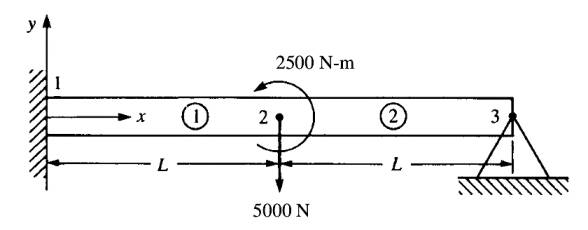
\includegraphics[width=10em]{phy_020_strs_06_01.jpg}

Mesela üstteki ilk resimde bir vidanın döndürülmesi görülüyor, bu durumda bir el
bir $T$ torku uygular. Bir arabanın tekerlek aksı, şaftı ya da gemilerin
pervanesine (propeller) dönüş ileten aks aynı davranışı sergiler.  Altta üçüncü
resimde görülen tork ilk nokta için $T_1 = P_1 d_1$ ile, ikincisi $T_2 = P_2
d_2$ ile hesaplanabilir.

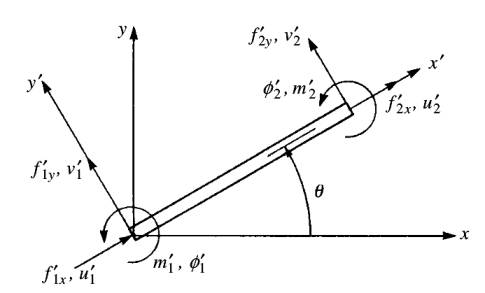
\includegraphics[width=15em]{phy_020_strs_06_02.jpg}

Burulma deformasyonunun mekaniğine biraz daha yakından bakalım. Bir çubuğu
$\phi(x)$ açısına gelecek şekilde büküyoruz, ve bu burulma bir $\gamma$ kaykılma
gerginliğine yol açıyor.

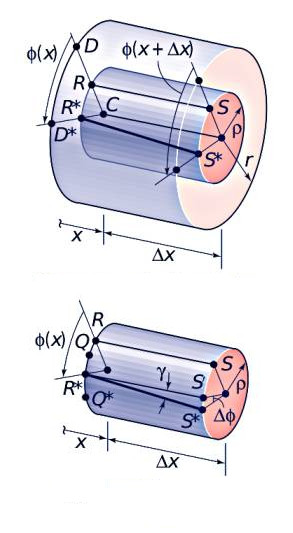
\includegraphics[width=10em]{phy_020_strs_06_03.jpg}

Üstteki ilk şekil çubuğun bir $x$ bağlamındaki bir parçasını gösteriyor,
altındaki ise o parçanın içindeki daha ufak yarıçaptaki bir parçasını [3, sf. 240]. 

$\gamma$ büyüklüğünü bulmak için üstteki resimde ikinci figure bakalım, $S^*$ ve
$S'$ arasındaki uzunluğu, $R^*$ ve $S'$ uzunluğuna bölersek (bu yapılabilir
çünkü ufak açılar sözkonusu ise tanjant hesabı aşağı yukarı açının kendisine
eşittir [2]) istenen sonucu bulabiliriz. Tabii $R^*S'$ uzunluğu $\Delta x$,
ve $S^*S'$ uzunluğu çember çevresinin ufak bir parçası, onu  $\rho \Delta \phi$
ile buluruz, bunları bir limit hesabı ile ifade edersek, ve $\Delta x \to 0$
iken

$$
\gamma = \lim_{\Delta x \to 0} \frac{S^*S'}{R^*S'} =
\lim_{\Delta x \to 0} \frac{\rho \Delta \phi}{\Delta x} =
\rho \frac{\ud \phi}{\ud x}
$$

O zaman eksenel yuvarlak olan bir birimin burumsal deformasyon için
gerginlik-yer değişim (strain-displacement) denklemi

$$
\gamma = \gamma(x,\rho) = \rho \frac{\ud \phi}{\ud x}
$$

$\phi$'in $x$'e göre türevi alınabildi çünkü formülü $x$'e bağlıdır, bunu
üstteki grafikte ilk figürde görüyoruz, $\phi(x)$ açısı $\phi(x+\Delta x)$
açısından farklı. Eğer $\phi$'yi formülsel olarak düşünsek herhalde $x$ arttıkça
ona lineer oranla artan bir açı büyüklüğü formülize edilebilirdi.



[devam edecek]

Kaynaklar

[1] Gere, {\em Mechanics of Materials}

[2] Bayramlı, {\em Normal Diferansiyel Denklemler, Trigonometri}

[3] Craig, {\em Mechanics of Materials}

\end{document}
